\documentclass{article}

\usepackage{CJKutf8}
\usepackage{multicol}
\usepackage[margin=2cm]{geometry}
\usepackage{listings}
\usepackage{graphicx}
\graphicspath{ {./img/} }

\title{\Large {HW1: Real-time Debugging of a HW-SW Platform}}
\author{學號:0711282 邱頎霖}
\date{}

\begin{document}
\begin{CJK*}{UTF8}{bsmi}
\setlength{\columnsep}{1cm}

\vspace*{-90pt}
    {\let\newpage\relax\maketitle}

\begin{multicols}{2}

\begin{center}
    \section*{INTRODUCTION}
\end{center}

\begin{flushleft}
    此次作業在原始\ Dhrystone 不做任何修改下所得到的\ DMIPS 為\ 0.72, \
    此篇\ report 中將會先透過反組譯所得到的組合語言、Aquila 架構 與\ Vivado waveform 進行分析, \ 
    找出當前的缺點後, 以組合語言嵌入\ Dhrystone 原始碼中實現優化的方法。 
\end{flushleft}

\begin{center}
    \section*{ANALYZE}
\end{center}
\begin{flushleft}
反組譯後可以獲得\ CODE. 1. 組合語言內容,搭配\ waveform 可以清楚且快速的知道哪些時候發生\ stall,\
觀察整個\ \textit{strcpy function} 後,\
可以知道主要發生\ stall 的指令為\ Fig. 1. 用紅線框選出來的兩個區塊。\newline
\end{flushleft}

% ===== start of stall date fetch =====
\begin{center}
    \subsection*{stall data fetch}
\end{center}
\begin{flushleft}
Fig. 1. 中第一個\ stall 區塊發生\ \textit{stall\_data\_fetch},\ 
而發生主要原因為\ \textit{core\_top.v} 中的\ finite state machine 中的
\end{flushleft}

\begin{center}
    \begin{lstlisting}[
        basicstyle=\footnotesize, 
    ]
            dS_nxt == d_WAIT
    \end{lstlisting}
\end{center}

\begin{flushleft}
往回追朔最終在 \ \textit{decode.v} 中找到導致 \ \textit{stall\_data\_fetch}\
發生的情況為:
\end{flushleft}

\begin{center}
    \begin{lstlisting}[
        basicstyle=\footnotesize, 
    ]
    assign re = rv32_load | rv32_amo; 
    assign we = rv32_store | rv32_fencei;
    \end{lstlisting}
\end{center}
\textit{decode.v}\ 會往後不斷傳遞給下一個\ pipeline stage,\
在 \ execute stage 將訊號輸入到\ memory stage 就會發生\ stall。\
總結, 以此次作業情況, 當要使用\ \textit{load} 或是 \ \textit{store}\ 
會\ stall 所有\ pipeline stage 1 cycle, 因此如果需要使用到這兩個指令時,\
\ stall 1 cycle 無法避免。

% ===== end of stall date fetch =====
\begin{center}
    \subsection*{stall data hazard}
\end{center}

\begin{flushleft}
    第二個\ stall 區塊除了發生上述的\ \textit{stall\_data\_fetch},
    還發生\ \textit{stall\_data\_hazard},\ data hazard 的產生源自\ pipeline 中某一指令使用到之前階段指令尚未產生的結果,\
    解決方法可以分為軟體方法與硬體方法。\\
    軟體方法分為:\
    \begin{enumerate}
        \item 重新排序程式碼使其沒有資料相依
        \item 暫停\ pipeline 使需要的結果產生後再執行
    \end{enumerate}
    硬體方法為:
    \begin{enumerate}
        \item forwarding: 通過拉線的硬體方式,將需要的資料提早送到前面的 pipeline stage
    \end{enumerate}
    需要特別注意的是使用\ forwarding 的方式如果遇到\ load-use instruction, 必須要\ stall 1 cycle,\
    如\ Fig. 2. 當要 load 資料時最少要等到\ memory stage 。\
    根據\ Aquila 原始碼中可以找到 \ \textit{stall\_data\_hazard} 發生的源頭為\
    \textit{decode.v}\, 為\ CODE. 2. 中的內容, \ \textit{re\_o} 表示上一筆指令是否為 load 指令,\
    \ \textit{rd\_addr\_o} 表示上一筆指令的目的暫存器, \

    \columnbreak
    % this is column break to split content

    \begin{flushleft}
        \begin{center}
            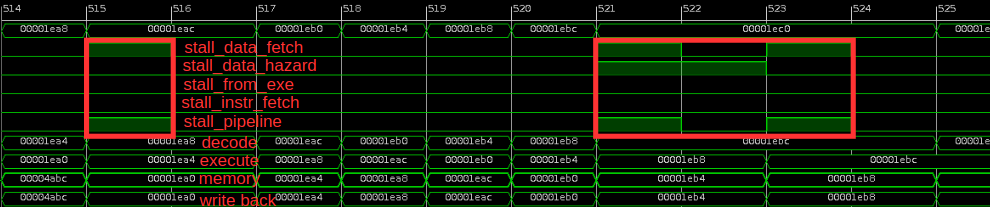
\includegraphics[width=8cm]{analyze}
            \small FIG. 1. waveform after executing strcpy in Dhrystone
        \end{center}
    \end{flushleft}
    \begin{center}
        \begin{lstlisting}[
            basicstyle=\footnotesize, 
        ]
00001ea0 <strcpy>:
    1ea0: 0005c783 lbu	a5,0(a1)
    1ea4: 00050713 mv	a4,a0
    1ea8: 00078c63 beqz	a5,1ec0 <strcpy+0x20>
    1eac: 00170713 addi	a4,a4,1
    1eb0: 00158593 addi	a1,a1,1
    1eb4: fef70fa3 sb	a5,-1(a4)
    1eb8: 0005c783 lbu	a5,0(a1)
    1ebc: fe0798e3 bnez	a5,1eac <strcpy+0xc>
    1ec0: 00070023 sb	zero,0(a4)
    1ec4: 00008067 ret
        \end{lstlisting}
        \small CODE. 1. strcpy assembly code
    \end{center}

    當上一筆指令為 load 指令且當前指令的來源暫存器與上一筆指令的目的暫存器相同時,\
    即為\ load-use instruction, 因此需要\ stall 1 cycle。\ 
    此處僅\ stall program counter 與\ fetch stage,\
    其他\ pipeline stage 仍要繼續執行。\
    根據\ FIG. 1.\
    我們可以驗證\ CODE. 1. 中的\ 1ebc 這條指令在 decode stage 時的確顯示\ data hazard\newline

    根據\ strcmp 的\ waveform Fig. 2. 後可以發現其缺點與\ strcpy 近乎相同,\
    都是含有 \ \textit{stall\_data\_fetch} 與 \ \textit{stall\_data\_hazard},\
    因此我的想法是將優化的方法同時套用到這兩個\ function 上理論上就可以比原始碼獲得更高的 DMIPS.\newline

    根據上面的分析, 可以知道\ load-use instruction 會導致額外\ stall 1 cycle,\
    然而不如 \ \textit{stall\_data\_fetch} 無法避免,\
    透過重新排列指令的方法可以將原本含有\ load-use instruction 給消除,\
    因此重新排列指令將會是本次實現優化的目標。

\end{flushleft}

\begin{flushleft}
    \begin{center}
        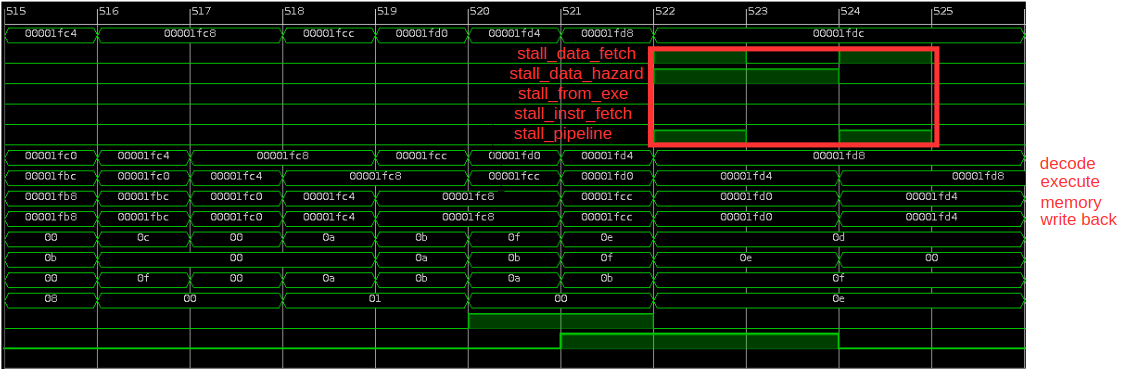
\includegraphics[width=8cm]{strcmp}
        \small FIG. 2. waveform after executing strcmp in Dhrystone
    \end{center}
\end{flushleft}

\begin{center}
    \begin{lstlisting}[
        basicstyle=\scriptsize, 
    ]
wire is_rs1_rd_same = (rs1_addr_o == rd_addr_o) 
    && (is_r_type || is_s_type || is_b_type 
        || is_i_type || is_fence || is_csr_type);
wire is_rs2_rd_same = (rs2_addr_o == rd_addr_o)
    && (is_r_type || is_s_type ||

assign is_load_hazard_o = 
    (is_rs1_rd_same | is_rs2_rd_same) && re_o;
    \end{lstlisting}
    \small CODE. 2. detect load-use instruction
\end{center}

\newpage

\begin{center}
    \section*{IMPLEMENTATION}    
    \subsection*{rescheduling}
\end{center}
\begin{flushleft}
    根據\ CODE. 1. 可以先觀察是否可以實現指令重排。\
    初始化會先將要複製的字元\ load 到暫存器\ \textit{a5},\
    判斷是否為空字串, 是的話\ branch 到\ 1ec0 處。\newline
    否的話執行下面直到字串完全複製結束:\newline
    \begin{enumerate}
        \item 移動要複製的字串指針\ \textit{a4} 指向下一個要填入複製字元的再後面一個位置\
        \item 移動被複製的字串指針\ \textit{a1},指向下一個要複製的字元\
        \item 將\ \textit{a5} 內容存到 \ \textit{a4} 指向位置的前一個位置\
        \item 將下一個要複製的字元\ load 到\ \textit{a5}\
        \item 利用\ \textit{a5} 內容判斷字串是否到尾端, 否的話繼續執行此迴圈\newline
    \end{enumerate}
    
    透過上面我們可以知道會發生\ load-use instruction 是因為第五步驟每次在判斷字串是否複製結束前,\
    必須先將下一個要複製的字元給\ load 出來, 因此不要讓\ load-use instruction 出現的方法就是\
    每次先做複製後在更新兩個字串的指標, CODE. 3. 為改動後的組合語言\newline

    對於\ strcmp 也使用同樣的概念進行優化。\ 
    原先\ strcmp function 的步驟如下:\newline
    \begin{enumerate}
        \item 初始化: 分別將兩個指標往前移動一個位置
        \item 比對過程: 將兩個指標往後移動一個位置, 並分別\ load 到暫存器, 進行比對
        \item 若非相同,\ return 相對應的數值;否則繼續第二步驟進行比對\newline
    \end{enumerate}
    原始碼中產生\ load-use instruction 的原因出現在\ 
    比對過程中將字元\ load 到暫存器後馬上接著比對,\
    因此優化方式為先指標指向的字元\ load 到暫存器中,\ 
    更新指標使兩個指標分別指向字串下一個位置,\
    再將\ load 到暫存器的字元比對後,\
    即可避免\ load-use instruction 的產生。\
    優化過後的內容如 CODE. 4. 所顯示,\
    也避免\ load-use instruction 的產生。
    
    \begin{center}
        \begin{lstlisting}[
            basicstyle=\scriptsize, 
        ]
00001ea0 <strcpy>:
    1ea0:	0005c783 lbu a5,0(a1)
    1ea4:	00050713 mv	a4,a0
    1ea8:	00078c63 beqz a5,1ec0 <copy_end>

00001eac <copy>:
    1eac:	00f70023 sb	a5,0(a4)
    1eb0:	00158593 addi a1,a1,1
    1eb4:	0005c783 lbu a5,0(a1)
    1eb8:	00170713 addi a4,a4,1
    1ebc:	fe0798e3 bnez a5,1eac <copy>

00001ec0 <copy_end>:
    1ec0:	00070023 sb	zero,0(a4)
    1ec4:	00008067 ret
        \end{lstlisting}
        \small CODE. 3. optimized strcpy
    \end{center}

    \columnbreak

    \begin{center}
        \begin{lstlisting}[
            basicstyle=\scriptsize, 
        ]
00001fb8 <strcmp>:
    1fb8:	0080006f j 1fc0 <compare>

00001fbc <str_end>:
    1fbc:	02078663 beqz	a5,1fe8 <ret_z>

00001fc0 <compare>:
    1fc0:	00054783 lbu	a5,0(a0)
    1fc4:	0005c703 lbu	a4,0(a1)
    1fc8:	00150513 addi	a0,a0,1
    1fcc:	00158593 addi	a1,a1,1
    1fd0:	fee786e3 beq	a5,a4,1fbc <str_end>
    1fd4:	fff00513 li	a0,-1
    1fd8:	00e7f463 bleu	a4,a5,1fe0 <ret_o>
    1fdc:	00008067 ret

00001fe0 <ret_o>:
    1fe0:	00100513 li	a0,1
    1fe4:	00008067 ret

00001fe8 <ret_z>:
    1fe8:	00000513 li	a0,0
    1fec:	00008067 ret
        \end{lstlisting}
        \small CODE. 4. optimized strcmp
    \end{center}    
\end{flushleft}

\begin{center}
    \subsection*{unroll}    
    根據觀察,\ Dhrystone 中\ string copy 每次都是\ copy 長度為 30 的字串,\
    因此可以利用將\ loop 展開的方式以增高效能, 避免了判斷是否字串已經複製完、\ branch 等指令,\
    當然在這裡寫死複製長度後\ string copy 在其他非字串長度為\ 30 的地方將會出現錯誤,\
    因此僅僅適用於此處。將\ string copy unroll 的過程如下:
    \begin{enumerate}
        \item 初始化, 包含使用另外一個指針進行複製的動作與第一次複製
        \item 重複\ 29 次複製
        \item 補\ 0 與\ return
    \end{enumerate}
\end{center}

\begin{center}
    \section*{SUMMARY}
    dsf
\end{center}

\section*{}

\end{multicols}

\end{CJK*}
\end{document}